\documentclass[a4paper,10pt]{scrartcl}

% Deutsche Umlaute (Mac)
\usepackage[applemac]{inputenc}

% Deutsche Umlaute (Windows)
%\usepackage[ansinew]{inputenc}

% Einbinden von Bildern
\usepackage{graphicx}

% SeitenflŠche etwas mehr ausnutzen
\usepackage{geometry}
\geometry{a4paper,left=30mm,right=30mm, top=1cm, bottom=3cm}

% Kein EinrŸcken bei zweispaltigen Bildunterschriften
\usepackage[normal]{caption}

% == Lottes Änderungen ===
\usepackage{todonotes}
\usepackage{hyperref}

% großer erster Buchstabe
\usepackage{lettrine}
\usepackage{graphicx}
\usepackage{caption}
\usepackage{subcaption}

% Glossary benutzen
\usepackage{glossaries}
\loadglsentries[main]{glossary}
\makeglossaries

% zeilenumbrüche in tabellen
\newcommand{\specialcell}[2][c]{%
  \begin{tabular}[#1]{@{}c@{}}#2\end{tabular}}

\begin{document}

% Titel
\title{Hybrid routing for the Internet of Things}
\subtitle{challenges and opportunities}
\author{Lotte Steenbrink}
\date{Wintersemester 2014/15}
\maketitle

\begin{abstract}
I am an abstract. Write me!

With the \gls{IoT}, new use cases and requirements for mobile mesh networks have begun to blossom. In order to meet these requirements, routing protocols are needed to manage connectivity and prepare the transport of packets. These protocols need to be able to adopt to a rapidly changing environment, and do so autonomously and efficiently. Because traditional approaches to routing may not be feasible for this task, \emph{hybrid roting protocols} have begun to resurface. This paper will introduce existing approaches to hybrid routing and aims to provide pointers on how to evolve them to make them a perfect fit for the IoT.

\end{abstract}

\section{Introduction}
\label{sec:Intro}
%==============================================================================
TODO

\subsection{What is the Internet of Things?}
\label{subsec:IoT}
%==============================================================================
The \gls{IoT} envisions autonomous communication between tiny computers installed in everyday objects such as furniture, toys, clothing, or tools with the goal of making them smarter and improving their user experience. IoT devices typically are very constrained devices with no constant power supply. Therefor, they need to be resourceful in terms of computation, storage, RAM and energy usage.
To communicate amongst each other, IoT nodes form spontaneous, wireless mesh networks.
The vision of the Internet of Things is rapidly becoming reality, and with its rise, new demands for routing protocols that serve these kinds of mesh networks surface which cannot be optimally served by either reactive or proactive routing protocols alone.\\
One example for this may be the lighting system in a smart home: Each lamp needs to maintain a stable connection to the control center of the house, forming a tree-like topology towards the sink node that is the central control. In addition to this, lamps may want to communicate spontaneously between each other, for example to create optimal lighting in the study when homeowners sit down at their desk.

\subsection{What is Hybrid Routing?}
\label{subsec:hybrid}
%==============================================================================
Hybrid Routing protocols combine two central routing paradigms into one protocol: Reactive and proactive routing. While reactive protocols stay idle until a route is needed and then \emph{react} to this demand, proactive protocols constantly monitor their network for peers and link qualities, (re-)calculating routes as they gather new data. The former class of protocols perform well in sparse, very mobile networks and save energy by generating less control overhead. The latter are best suited for networks with high demands in terms of throughput, reliability and latency.\\
Hybrid routing protocols aim to adjust their routing strategy from proactive to reactive and back depending on the circumstances: Routes or areas that are deemed important or see a lot of traffic require proactive attention, while sparsely, less important or very mobile areas or routes are best served reactively.\\
In th example of section \ref{subsec:IoT}, all lamps would maintain a proactive route towards the control center, while inter-lamp communication may be set up reactively.

\section{Related work}
\label{sec:related_work}
%==============================================================================
\todo{Talk about the past, mostly. talk about areas of research we can steal from.
briefly mention experimental work, esp emmanuels, reference \ref{sec:experiments}.}

Most research on hybrid routing protocols stems from an era where wireless mesh routing was at its very beginning. This meant that the building blocks for hybrid routing, namely proactive and reactive routing protocols, were under construction themselves. While proactive and reactive protocols were developed and examined, research in hybrid routing stalled until a more thorough understanding of proactive and reactive has been reached.\\
This has since been achieved: The \gls{IETF} has standardized \gls{OLSR}, OLSRv2  and \gls{AODV}, AODVv2 is on its way to become a standard, and \gls{LOADng} has been deployed in large-scale energy grid networks (TODO: quelle). The body of experience with both reactive and proactive protocols has grown, and research towards hybrid protocols has begun to blossom \cite{baccelli_p2p_rpl} \cite{HYMAD}\\

But while this milestone has been reached, the amount of protocols of any kind specifically targeted at IoT-like environments is very small. By the time of this writing, the \gls{RPL} is the only dedicated IoT protocol available, and it cannot cover the entire diverse set of requirements that can be found under the umbrella term of ``Internet of Things''. Thus, it is necessary to evaluate protocols designed for environments that share some characteristics with the Internet of Things and may be customized to be a good fit, such as \glspl{DTN}, \glspl{MANET} and, to a certain extent, \glspl{VANET}.\\

The goal of this paper is thus to explore how hybrid routing can be advanced with the \gls{IoT} in mind, building on the foundation which research on \gls{MANET} routing of the past 15 years has built.\\ 
The rest of this paper is organized as follows. \todo{TODO! double-check!}

\section{Key aspects of Hybrid Routing Protocols}
\label{sec:key_aspects}
%==============================================================================
All hybrid protocols discussed in section \ref{sec:related_work} share common approaches, some of which fundamentally shape the way a routing protocol sees and serves a network. The goal of this section is to identify these key aspects and discuss them with regard to the requirements of IoT environment.

\subsection{Scope}
\label{subsec:scope}
%==============================================================================

\begin{figure}
        \centering
        \begin{subfigure}[b]{0.5\textwidth}
                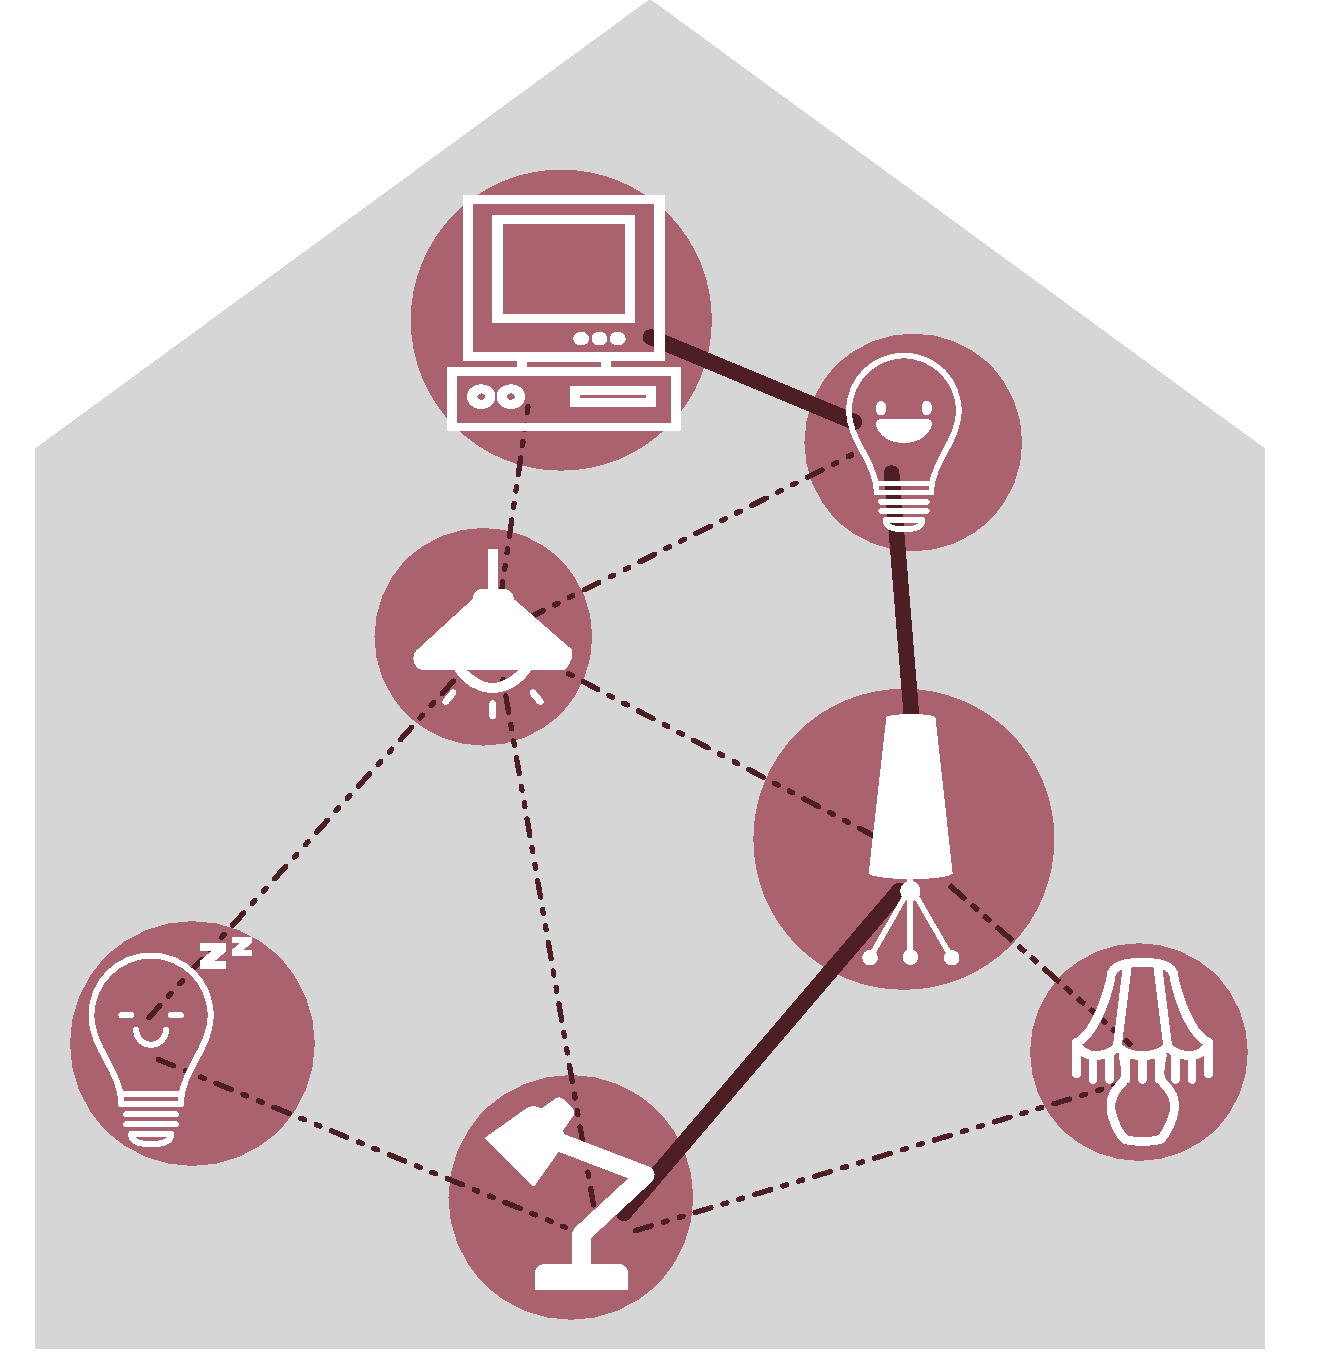
\includegraphics[width=\textwidth]{../images/route_centered_example}
                \caption{Example of a route-centered network: lights and control center in a smart home.}
                \label{fig:rc_img}
        \end{subfigure}%
        ~ %add desired spacing between images, e. g. ~, \quad, \qquad, \hfill etc.
          %(or a blank line to force the subfigure onto a new line)
        \begin{subfigure}[b]{0.5\textwidth}
                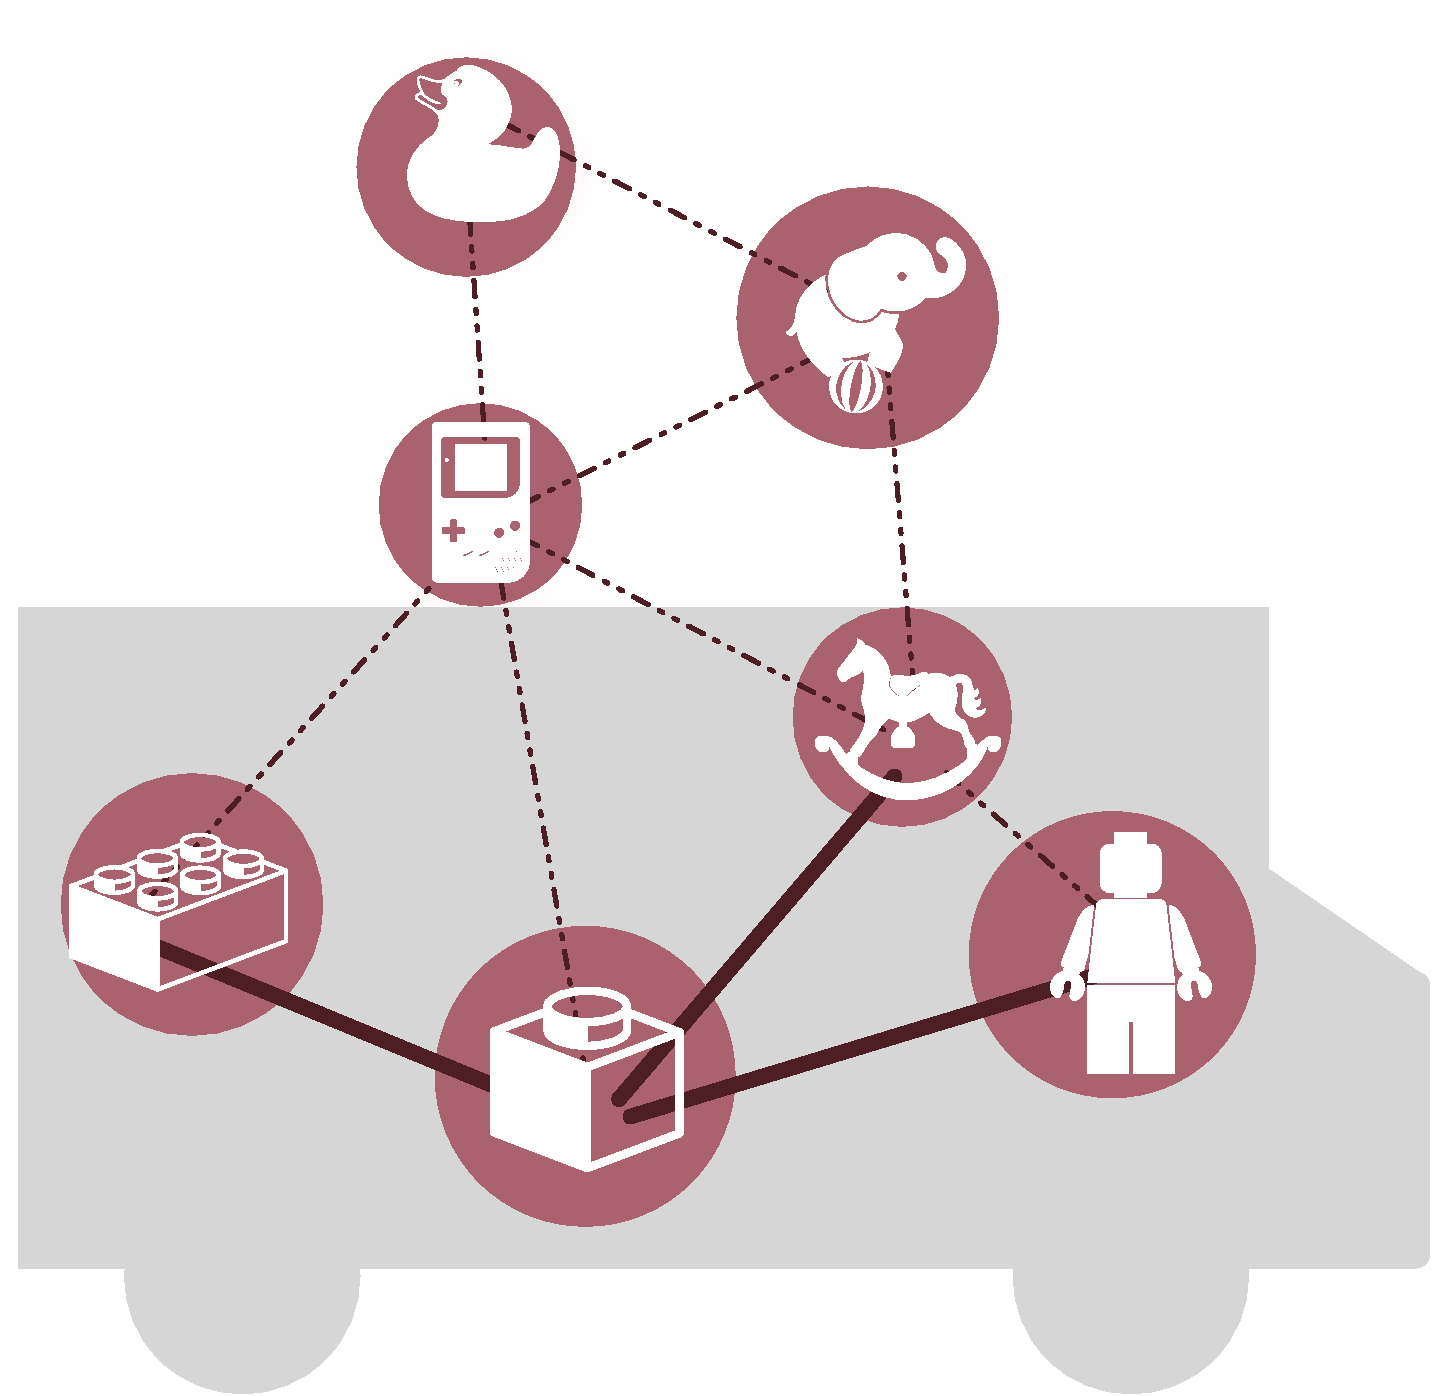
\includegraphics[width=\textwidth]{../images/area_centered_example}
                \caption{Example of an area-centered network: Goods in a delivery truck and warehouse}
                \label{fig:ac_img}
        \end{subfigure}
        \caption{Application Scenarios for hybrid routing protocols}\label{fig:scope}
\end{figure}

Hybrid protocols differ in the way they prioritize routes and decide which of them should be maintained proactively or set up reactively. There are two approaches to this, which this paper dubs the \emph{route-centered} and the \emph{area-centered} approach repectively.\\

The \emph{route-centered} approach serves networks in which some nodes, near or far, are more important than others. This is illustrated by fig. \ref{fig:rc_img}, which shows the different lamps of a house and the house's control center. Each lamp needs a stable connection to this control center, be it to switch on/off occasionally to confuse burglars, or exchange status info and configurations. Thus, this connection is maintained proactively, as indicated in the diagram by the thick straight line. Additionally, they may want to communicate with each other upon user interaction. Because this happens spontaneously and sparsely, the connections amongst all lamps are set up reactively, as indicated by the dotted lines.\\
Protocols with an \emph{area-centered} approach assume all nodes are equal in principle, but nearby nodes are both more important than nodes which are farther away and know their neighborhood best. They cluster the network into so-called ``routing zones''. Nodes that are in the same zone maintain their connections among each other proactively, and routes towards nodes from foreign zones are established reactively. \todo{write about intra-zone routing, border nodes etc}
One example application for this may be a warehouse as illustrated in \ref{fig:ac_img} whose goods (or their packaging) are equipped with IoT hardware. Employees are thus able to tell details about the stock simply by asking their scanner, which communicated with the other IoT devices. In case a truckload of new goods arrives, \todo{write less fussy}

\todo{vor- und nachteile?}

\subsection{Architecture}
\label{subsec:architecture}
%==============================================================================
Because hybrid protocols incorporate proactive and reactive protocols as building blocks, their design in terms of architecture-- how it all goes together-- may be more than just a sequence of instructions. \todo{gibt es uberhaupt ``pure'' frameworks?}
They may either be \emph{monolithic protocols} which have a reactive and a proactive component firmly in place. Oftentimes, these components are variations of well-known proactive and reactive protocols, customized to improve the hybrid protocol's overall performance or decrease traffic- or computational overhead. For example, \cite{baccelli_p2p_rpl} piggybacks reactive control traffic onto already existing, proactive RPL messages, thus avoiding unnecessary traffic and saving battery life. \todo{mehr Beispielprotokolle auflistem}
This bears great potential for optimization, but complicates code re-use and the deployment of updates.\\
Or, hybrid solutions may be organized as a mere \emph{framework} with which can be used to bring together different proactive or reactive protocols. Many existing hybrid solutions such as SHARP, Node-Centric Hybrid Routing and HYMAD chose this route, but with a twist: one component, for example the reactive protocol, is fixed, while the proactive protocol can be exchanged at will. This architecture allows for a great deal of flexibility: If a new version of a protocol that is in use surfaces, it can be adopted quickly. The same with alternative protocols which prove to serve some or all use-cases better. Existing implementations of well-known proactive or reactive protocols can be integrated and re-used.
A hybrid framework bears the possibility to be customized for certain deployments, because the most suitable proactive and reactive protocols for the task may be picked and combined seamlessly.
Of course, this comes at the cost of lightweightedness: Approaches which are very flexible usually produce a higher amount of overhead. Additionally, if preexisting specifications and implementations are used, it may be hard to optimize them in terms of size and computational or traffic overhead.


%- flexibility, esp. as IoT is relatively new \& broad
%- lightweightness
%- ability to adopt to changes in underlying protocols
%- customizability? (depending on deployment)

\subsection{Existing Protocols}
\label{subsec:existing_protocols}
%-------------------------------------------------------------------------------
An Overview over all existing hybrid routing protocols for \glspl{MANET} and \glspl{DTN}\todo{was ist mit vanets?}
can be found in table \ref{fig:overview}. In the following, a short introduction to each protocol and its characteristic mechanisms will be provided.

\subsubsection{\gls{ZRP}}
\label{subsec:zrp}
%...............................................................................
The Zone Routing Protocol was originally developed for \glspl{MANET} and is one of the most-referenced and -extended hybrid routing protocols to date. It was originally described in an Internet-draft which expired on January 2003\cite{ZRP-Draft}.
It clusters nodes into so-called \emph{Routing Zones}, which adapt their diameter to the network's degree of mobility and traffic density. Routes inside these routing zones are discovered and maintained in a proactive fashion. In addition to the topology inside their zone, nodes are also aware of topology which all routing zones form.
To find routes to nodes in foreign routing zones, the reactive protocol makes use of a technique similar so some multicast routing approaches. The so-called \gls{BRP}\cite{draft-ietf-manet-zone-brp} protocol constructs a \emph{bordercasting} tree between all routing zones, and forwards the packet along the tree to one \emph{bordercasting node} per routing zone. Each bordercasting node will know if the target of the route discovery is in their routing zone, since the zones are maintained with a proactive protocol. If this is the case, it reports this to the source node, and the data exchange begins. If it is not the case, it forwards the packet. This way, traffic overhead is avoided.\\
The draft describes ZRP as a routing \emph{framework}, but describes its own proactive and reactive frameworks, namely the \gls{IARP}\cite{draft-ietf-manet-zone-iarp} for proactive routing inside routing zones, and the \gls{IERP}\cite{draft-ietf-manet-zone-ierp} to discover routes between zones reactively.\\
There are two extensions of ZRP: the \gls{TZRP}\cite{TZRP} and the \gls{IZR}\cite{IZR}. \todo{do I need to elaborate here?}

\subsubsection{\gls{ZHLS}}
\label{subsec:zhls}
%...............................................................................
ZHLS is a hierarchical, GPS-based roting protocol. 
ZHLS clusters all nodes into non-overlapping routing zones based on their location. These clusters form a hierarchy, with the nodes at its very bottom.
On startup, each node determines their location and joins the zone which spans across the area they're in. Route discovery within the zones is done in a proactive fashion. Whenever a packet needs to travel outside the cluster, it is routed along the zone hierarchy. Because there are no cluster heads, a lot of flooding happens. \todo{disentangle the general WTFness of this protocols's operation}
This protocol design bears the dangerous assumption that physical proximity guarantees near-optimal connectivity, which has been debunked by \cite{mistaken-axioms}. \todo{go into troubles of georouting?}

\subsubsection{Node-Centric Hybrid Routing}
\label{subsec:nchr}
%...............................................................................


\subsubsection{\gls{SHARP}}
\label{subsec:sharp}
%...............................................................................

\subsubsection{\gls{WARP}}
\label{subsec:warp}
%...............................................................................

\subsubsection{\gls{HYMAD}}
\label{subsec:hymad}
%...............................................................................
Just like ZRP and ZHLS\todo{and more?}, nodes form proactively maintained zones. The difference to all previously named protocols is that HYMAD borrows its approach to inter-zone roting not from traditional \gls{MANET} schemes, but from Delay-Tolerant Networks (DTN), where nodes store data until they move and meet other nodes with which they can communicate (this is called \emph{store-and-forward}).


\begin{table*}[t]
    \begin{tabular}{p{0.6\textwidth}|l|l|l}
        Name & Scope & Architecture & Published \\
        \hline
        Node-Centric Hybrid Routing \cite{Roy_nodecentric} & Route & Framework & 2002 \\ % proactive fixed
        \gls{SHARP}\cite{SHARP} & Route & Framework & 2003 \\ %TODO: only for reactive!
        P2P extension\cite{RFC-6997} of RPL\cite{RFC-6550} & Route & Protocol & 2013\\
        \gls{ZRP} \cite{ZRP-Draft} and extensions \cite{TZRP} \cite{IZR} & Area & Protocol & 2002/2004\\
        \gls{WARP}\cite{WARP} & Area & Protocol & 2002\\
        \gls{ZHLS}\cite{ZHLS} & Area & Protocol & 1999\\
        \gls{HYMAD}\cite{HYMAD} & Area & Framework & 2010\\ % Only DTN protocol is variable!
    \end{tabular}
    \caption{Overview over existing hybrid protocols}
    \label{fig:overview}
\end{table*}

\section{Experimental work}
\label{sec:experiments}
%==============================================================================
Most research concerning hybrid routing protocols stems from a time where large testbeds were not very feasible and simulations were conducted instead. \todo{sources, examples} Thus, publications documenting real-world experience with hybrid deployments are rare.\\

\cite{gomez_NSTAODV_eval} has evaluated the reactive AODVv2 protocol for IEEE 802.15.4. networks, a technology widely used in IoT deployments, as early as in 2006. However, the ``real environment'' used consists of 4-7 nodes, arranged in different topologies with a per-node distance of 12 cm. While a careful evaluation of simplified topologies is invaluable when examining new approaches, these findings can not provide us with information on the performance of (NST-)AODV in large scale, production IoT deployments.
\cite{baccelli_p2p_prl} reports about testbed experiences with P2P-RPL, comparing its performance in comparison to pure RPL in terms of route length and percentage of routes traversing the root node.
In \cite{WARP}, WARP is compared to OLSR in experiments with a ``real'' network, which turns out to consist of 14 unidentified laptops connected to an unspecified number of stationary PCs over ethernet. This research is from 2002, a time when WiFi hardware wasn't necessarily standard in consumer-grade laptops.\\

While simulations have proven to be useful for protocol design and evaluation, there are two main problems to a simulation-based approach: \todo{find a source for this. STAT.}
\begin{enumerate}
\item A simulation is only as good as its model. Without data from ``real world'' experiments, verifying that a model represents real conditions satisfactorily is hard.\todo{impossible is too harsh, non?}
\item Even when the model is adequately accurate, it can never account for the unforeseen quirks which will be encountered in a real environment. Especially in wireless networking, a node's environment (i.e. flying bids, surfaces reflecting differently based on time or weather conditions, unforeseeable radio propagation...) is a big and unforeseeable influence.
\end{enumerate}
In conclusion, experiences from real-world experiments or deployments are vital to fully understand the challenges of hybrid IoT routing and assess the solutions at hand. Because the opportunity to deploy experimental software on productive systems is rarely given, more and more testbeds have been established in recent years. \cite{testbed-survey} provides a requirement analysis for IoT-ready testbeds. It concludes that in order to be suitable for meaningful research, testbeds need to offer the following features to their users:
\begin{description}
\item[Experimentation:] The ability to specify, interact with, monitor, and repeat an experiment in a straightforward way. Additionally, the ability to run an experiment through simulation, with conditions similar to the testbed, should be given.  
\item[Hardware Features:] The hardware provided should be heterogeneous, with various capabilities and sensor types. The number of available devices should be possibly in the hundreds, with the possibly to add more recent devices in the future. In case of testbeds that span across several sites, the possibility of federating them into a big network should be given. The hardware should be subject to regular maintenance.
\item[Mobility:] Devices of the testbed should be able to move around in various patterns with the help of robotic and automation systems.
\item[Software management \& tools:] Simulation scenario configuration, may it be mobility patterns, hardware configurations, or low-level device control, should be easily accessible.
\end{description}
Based on this analysis, it provides an overview over existing facilities and their features. The two biggest testbeds, IoT-Lab\footnote{\url{https://www.iot-lab.info}} and smartsantander\footnote{\url{http://www.smartsantander.eu}} feature between 2,728 and 20,000 nodes and, even though their primary target are \glspl{WSN}, provide mobility through toy trains (IoT-Lab) or public buses (senslab). The latter has an impact on the reproduceability of experiments and limits the influence an experiment designer has on mobility patterns.
% + conclusion -> use iot-lab?

\section{Suitability for the IoT}
\label{sec:suitability}
%==============================================================================
Because most of the discussed hybrid protocols have not been designed for the IoT, not all of their key characteristics may be suitable for such a deployment. As discussed in \ref{sec:key_aspects}, routes can be categorized to be either route- or area-centered in terms of scope, and either frameworks or monolithic protocols in terms of architecture. 
Some of these aspects may foster behavior which is more suitable for the IoT than others.
Experience with both hybrid protocols and IoT environments \todo{das kann doch nicht wahr sein.. noch mal nach papers suchen!}
is rare, as detailed in \ref{sec:experiments}, so all statements about suitability have to be taken as educated guesses rather than hard truths.


\section{Conclusion}
\label{sec:conclusion}
%==============================================================================
translate old shit. Framework good, protocol bad. scope depends on deployment. framework may be able to accommodate that too. simulations mostly suck. real-world experiences are rare. hooray for testbeds! Use IoT-Lab!

\section{Outlook}
\label{sec:outlook}
%==============================================================================
figure out ways to slim down frameworks.
get real-world experiences. verify vermutungen oder auch nicht. so much to do!

\printglossaries

{\small
\bibliographystyle{ieeetr}
\bibliography{ausarbeitung}
}


\end{document}